\chapter{Arhitektura i dizajn sustava}
		
	Za arhitekturu sustava odabrali smo klasičan klijent-server pristup. \\
	
	\textbf{Klijent}\\
	Strana klijenta je web stranica izgrađena u programskom jeziku JavaScript uz pomoć biblioteke React. Odabrali smo ovu tehnologiju jer je React danas najkorištenija biblioteka za razvoj web stranica i kao takva nudi najbolji ekosustav funkcionalnosti i podrške. Korišteno razvojno okruženje je VScode. Zadatak klijenta je slanje zahtjeva prema serveru koji ih zatim obrađuje. Svi zahtjevi se šalju pomoću HTTP POST metode i šalju se u JSON formatu prema serveru.\\
	
	\textbf{Server}\\
	Za server stranu odabrali smo programski jezik Javu i razvojno okruženje \textit{Spring Boot}. \textit{Spring Boot} smo odabrali jer je standardno razvojno okruženje za jezik Javu, a Javu smo odabrali kako bismo na prirodan način mogli sustav implementirati koristeći objektno orijentiranu paradigmu. Za razvoj serverskog koda korišten je alata Intellij IDEA. \textit{Spring Boot} nam također nudi neke dodate pogodnosti kao što je proširenje \textit{Spring Security} koje znatno olakšava proces implementacije sigurnog i točnog procesa prijave i registracije korisnika. Server prima zahtjeve od klijenta u JSON formatu i pretvara te zahtjeve u Java objekte nad kojima izvršava daljnje operacije. Kada server obradi zahtjev šalje natrag HTTP odgovor s odgovarajućim statusnim kodom kako bi klijent znao je li operacija uspjela ili nije.
		

		

				
		\section{Baza podataka}
			
		 Kao sustav za upravljanje bazama podataka odabrali smo PostgreSQL. Implementacija naše PostgreSQL baze podataka obuhvaća nekoliko ključnih elemenata, uključujući organizaciju podataka u tablicama i uspostavljanje veza između tablica radi složenih upita. Baza podatka sastoji se od slijedećih entiteta: 
		
		\begin{packed_item}
			\item KLINIKA
			\item SMJEŠTAJ
			\item PRIJEVOZNIK
			\item VOZILO
			\item KORISNIK
			\item PUTOVANJE
		\end{packed_item}
		
			\subsection{Opis tablica}
			
				\textbf{KLINIKA}\hspace{0.5cm}Entitet KLINIKA sadrži informacije o ID-u klinike, nazivu i adresi. Prema tome, entitet KLINIKA posjeduje sljedeće atribute: IDKlinika, naziv i adresa. Entitet KLINIKA je u vezi \textit{One-to-Many} s entitetom SMJESTAJ preko atributa IDKlinika i u vezi \textit{One-to-Many} s enitetom PUTOVANJE preko atributa IDKlinika. Također je u \textit{One-to-Many} vezi s enitetom PUTOVANJE preko atributa adresa.
				
				\begin{longtblr}[
					label=none,
					entry=none
					]{
						width = \textwidth,
						colspec={|X[6,l]|X[6, l]|X[20, l]|}, 
						rowhead = 1,
					} %definicija širine tablice, širine stupaca, poravnanje i broja redaka naslova tablice
					\hline \SetCell[c=3]{c}{\textbf{KLINIKA}}	 \\ \hline[3pt]
					\SetCell{LightGreen}IDKlinika & INT	& Identifikacijski ključ klinike	\\ \hline
					naziv	& VARCHAR & Naziv klinike\\ \hline 
					adresa & VARCHAR & Adresa klinike\\ \hline 
				\end{longtblr}
				
				\textbf{SMJESTAJ}\hspace{0.5cm}Entitet SMJESTAJ sadrži podatke o ID-u smještaja, tipu stana, kategoriji opremljenosti, adresi kao i vremenskom periodu dostupnosti za korištenje. Sukladno tome, entitet SMJESTAJ posjeduje sljedeće atribute: IDSmjestaj, tip, kategorija, adresa i dostupnost. Entiet SMJESTAJ je u vezi  \textit{Many-to-One} s entitetom KLINIKA preko atributa IDKlinika i u vezi  \textit{One-to-Many} s enitetom PUTOVANJE preko atributa IDPutovanje. Također je u \textit{One-to-Many} vezi s enitetom PUTOVANJE preko atributa adresa.
				
				\begin{longtblr}[
					label=none,
					entry=none
					]{
						width = \textwidth,
						colspec={|X[6,l]|X[6, l]|X[20, l]|}, 
						rowhead = 1,
					} %definicija širine tablice, širine stupaca, poravnanje i broja redaka naslova tablice
					\hline \SetCell[c=3]{c}{\textbf{SMJESTAJ}}	 \\ \hline[3pt]
					\SetCell{LightGreen}IDSmjestaj & INT	&  Identifikacijski ključ smještaja	\\ \hline
					tip	& VARCHAR &  Tip stana\\ \hline 
					kategorija & VARCHAR & Kategorija opremljenosti  \\ \hline 
					adresa & VARCHAR	&  Adresa smještaja\\ \hline 
					dostupnost & INTERVAL	&  Vremenski period dostupnosti za korištenje\\ \hline 
					\SetCell{LightBlue} IDKlinika & INT	&  Identifikacijski ključ klinike  	\\ \hline 
				\end{longtblr}
				
				\textbf{PRIJEVOZNIK}\hspace{0.5cm}Entitet PRIJEVOZNIK sadrži informacije o ID-u prijevoznika, kontaktnim podacima i o radnom vremenu u kojem je prijevoznik raspoloživ. Prema tome, entitet PRIJEVOZNIK posjeduje sljedeće atribute: IDPrijevoznik, kontakt i radnoVrijeme. Entitet PRIJEVOZNIK je u vezi \textit{One-to-Many} s entitetom VOZILO preko atributa IDPrijevoznik i u vezi \textit{One-to-Many} s enitetom PUTOVANJE preko atributa IDPrijevoznik.
				
				
				\begin{longtblr}[
					label=none,
					entry=none
					]{
						width = \textwidth,
						colspec={|X[6,l]|X[6, l]|X[20, l]|}, 
						rowhead = 1,
					} %definicija širine tablice, širine stupaca, poravnanje i broja redaka naslova tablice
					\hline \SetCell[c=3]{c}{\textbf{PRIJEVOZNIK}}	 \\ \hline[3pt]
					\SetCell{LightGreen}IDPrijevoznik & INT	& Identifikacijski ključ prijevoznika	\\ \hline
					kontakt	& VARCHAR &  Kontaktni podatci prijevoznika	\\ \hline 
					radnoVrijeme & TIME & Radno vrijeme u kojem su prijevoznici raspoloživi  \\ \hline 
				\end{longtblr}
				
				\textbf{VOZILO}\hspace{0.5cm}Entitet VOZILO sadrži informacije o ID-u vozila, vrsti i kapacitetu prijevoznog sredstva. Prema tome, entitet VOZILO posjeduje sljedeće atribute: IDVozilo, vrsta i kapacitet. Entitet VOZILO je u vezi \textit{Many-to-One} s entitetom PRIJEVOZNIK preko atributa IDPrijevoznik.
				
				\begin{longtblr}[
					label=none,
					entry=none
					]{
						width = \textwidth,
						colspec={|X[6,l]|X[6, l]|X[20, l]|}, 
						rowhead = 1,
					} %definicija širine tablice, širine stupaca, poravnanje i broja redaka naslova tablice
					\hline \SetCell[c=3]{c}{\textbf{VOZILO}}	 \\ \hline[3pt]
					\SetCell{LightGreen}IDVozilo & INT	&  Identifikacijski ključ vozila	\\ \hline
					vrsta	& VARCHAR & Vrsta vozila\\ \hline 
					kapacitet & VARCHAR & Kapacitet vozila\\ \hline 
					\SetCell{LightBlue} IDPrijevoznik & INT	& Identifikacijski ključ prijevoznika   	\\ \hline 
				\end{longtblr}
				
				\textbf{KORISNIK}\hspace{0.5cm}Entitet KORISNIK sadrži informacije o ID-u korisnika, imenu, prezimenu, kontaktnim podacima i preferencijama vezanim uz veličinu i kvalitetu smještaja. Prema tome, entitet KORISNIK posjeduje sljedeće atribute: IDKorisnik, ime, prezime, kontakt i preferencije. Entitet KORISNIK je u vezi \textit{One-to-Many} s enitetom PUTOVANJE preko atributa IDKorisnik.
				
				\begin{longtblr}[
					label=none,
					entry=none
					]{
						width = \textwidth,
						colspec={|X[6,l]|X[6, l]|X[20, l]|}, 
						rowhead = 1,
					} %definicija širine tablice, širine stupaca, poravnanje i broja redaka naslova tablice
					\hline \SetCell[c=3]{c}{\textbf{KORISNIK}}	 \\ \hline[3pt]
					\SetCell{LightGreen}IDKorisnik & INT	&  Identifikacijski ključ korisnika	\\ \hline
					ime	& VARCHAR & Ime korisnika	\\ \hline 
					prezime & VARCHAR & Prezime korisnika \\ \hline
					kontakt & VARCHAR & Kontakt korisnika \\ \hline 
					preferencije & VARCHAR	& Preferencije vezane uz veličinu i kvalitetu smještaja\\ \hline 
				\end{longtblr}
				
				\textbf{PUTOVANJE}\hspace{0.5cm}Entitet PUTOVANJE sadrži informacije o ID-u putovanja, vremenu i smjeru putovanja. Prema tome, entitet PUTOVANJE posjeduje sljedeće atribute: IDPutovanje, vrijeme i smjer. Entitet PUTOVANJE j u vezi \textit{Many-to-One} s enitetom KLINIKA preko atributa IDKorisnik, u vezi \textit{Many-to-One} s enitetom SMJESTAJ preko atributa IDSmjestaj, u vezi \textit{Many-to-One} s enitetom KORISNIK preko atributa IDKorisnik, u vezi \textit{Many-to-One} s enitetom PRIJEVOZNIK preko atributa IDPrijevoznik. Atributi adresa1 i adresa2 su atributi iz kojih saznajemo adresu polaska ili dolaska u ovisnosti o smjeru koji može biti 1 ili 0. Entitet PUTOVANJE u vezi je \textit{Many-to-One} s enitetom KLINIKA preko atributa adresa1, u vezi \textit{Many-to-One} s enitetom SMJESTAJ preko atributa adresa2.
				
				\begin{longtblr}[
				label=none,
				entry=none
					]{
						width = \textwidth,
						colspec={|X[6,l]|X[6, l]|X[20, l]|}, 
						rowhead = 1,
					} %definicija širine tablice, širine stupaca, poravnanje i broja redaka naslova tablice
					\hline \SetCell[c=3]{c}{\textbf{PUTOVANJE}}	 \\ \hline[3pt]
					\SetCell{LightGreen}IDPutovanje & INT	&  Identifikacijski ključ putovanja	\\ \hline
					vrijeme	& TIME &  Vrijeme putovanja	\\ \hline 
					smjer & INT &  Smjer u kojem se putovanje izvodi \\ \hline 
					\SetCell{LightBlue} adresa1 & VARCHAR	&  Adresa klinike\\ \hline
					\SetCell{LightBlue} adresa2 & VARCHAR	& Adresa smještaja\\ \hline 
					\SetCell{LightBlue} IDKorisnik & INT	&  Identifikacijski ključ korisnika	\\ \hline 
					\SetCell{LightBlue} IDKlinika & INT	& Identifikacijski ključ klinike	\\ \hline
					\SetCell{LightBlue} IDPrijevoznik & INT	& Identifikacijski ključ prijevoznika	\\ \hline
					\SetCell{LightBlue} IDSmjestaj & INT	& Identifikacijski ključ smještaja	\\ \hline
				\end{longtblr}
				
			\eject
			
			\subsection{Dijagram baze podataka}
					
				\begin{figure}[htbp]
					\centering
					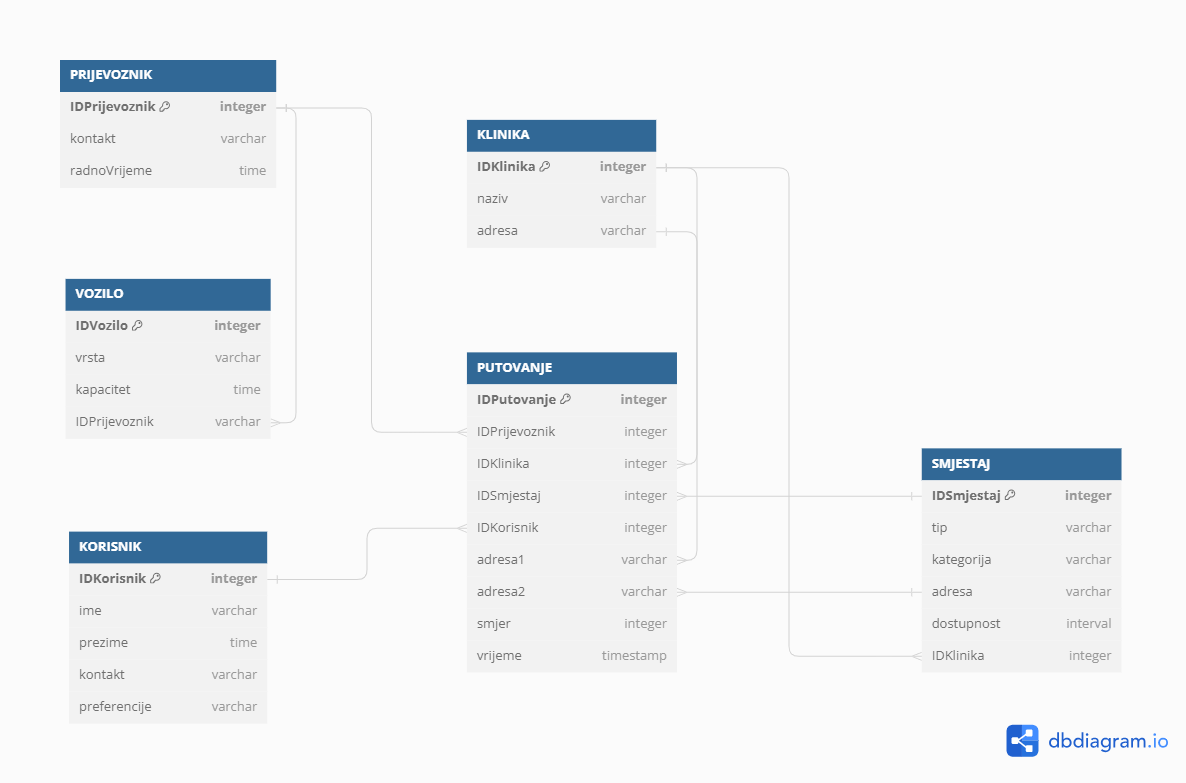
\includegraphics[width=0.9\textwidth]{slike/bazaPodataka.png}
					\caption{Relacijska shema baze podataka}
					\label{fig:bazaPodataka}
				\end{figure}
				
			
			\eject
			
			
		\section{Dijagram razreda}
		

			Na slikama 4.2, 4.3, 4.4 i 4.5 prikazani su razredi za implementaciju funkcionalnosti prijave i registracije korisnika. Na slici 4.2 prikazan je razred \textit{AuthController} koji služi prihvaćanju HTTP zahtjeva od strane klijenta i to specifično za URL \textit{/auth/**}. Metode \textit{login()} i \textit{register()} služe kao URL-ovi \textit{/auth/login} i \textit{/auth/register} na koje se šalju JSON objekti za prijavu administratora i registraciju novog administratora.
			
			\begin{figure}[htbp]
				\centering
				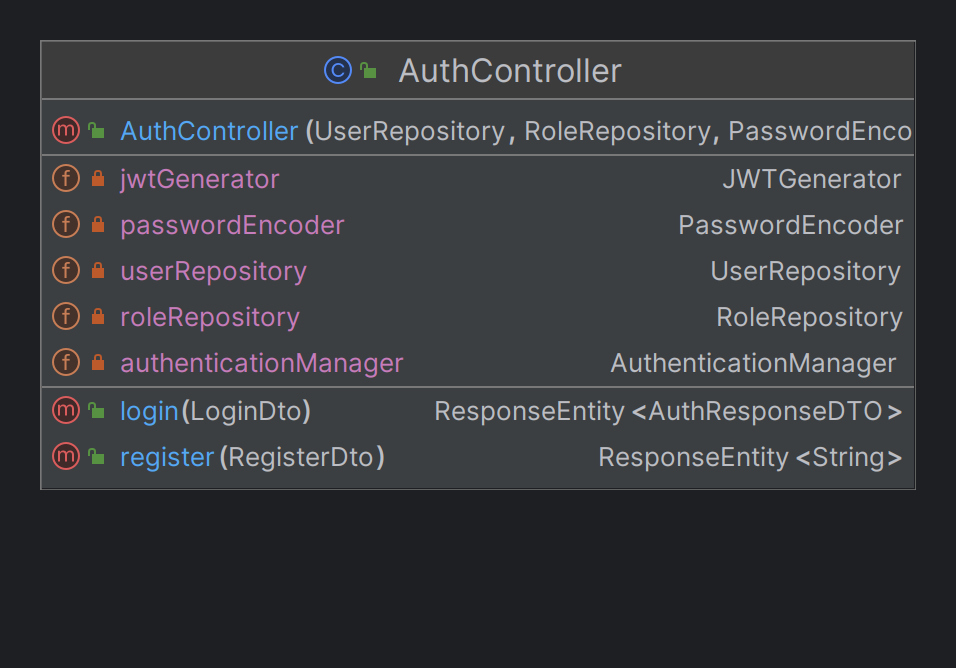
\includegraphics[width=0.9\textwidth]{slike/controllersUML}
				\caption{UML dijagram paketa \textit{Controllers}}
				\label{fig:controllersUML}
			\end{figure}
			
			Slika 4.3 prikazuje paket DTO koji služi za pretvaranje JSON objekata koji stižu na određenu rutu i Java objekt i za pretvaranje Java objekata u JSON odgovore koje klijent razumije.
			
			\begin{figure}[htbp]
				\centering
				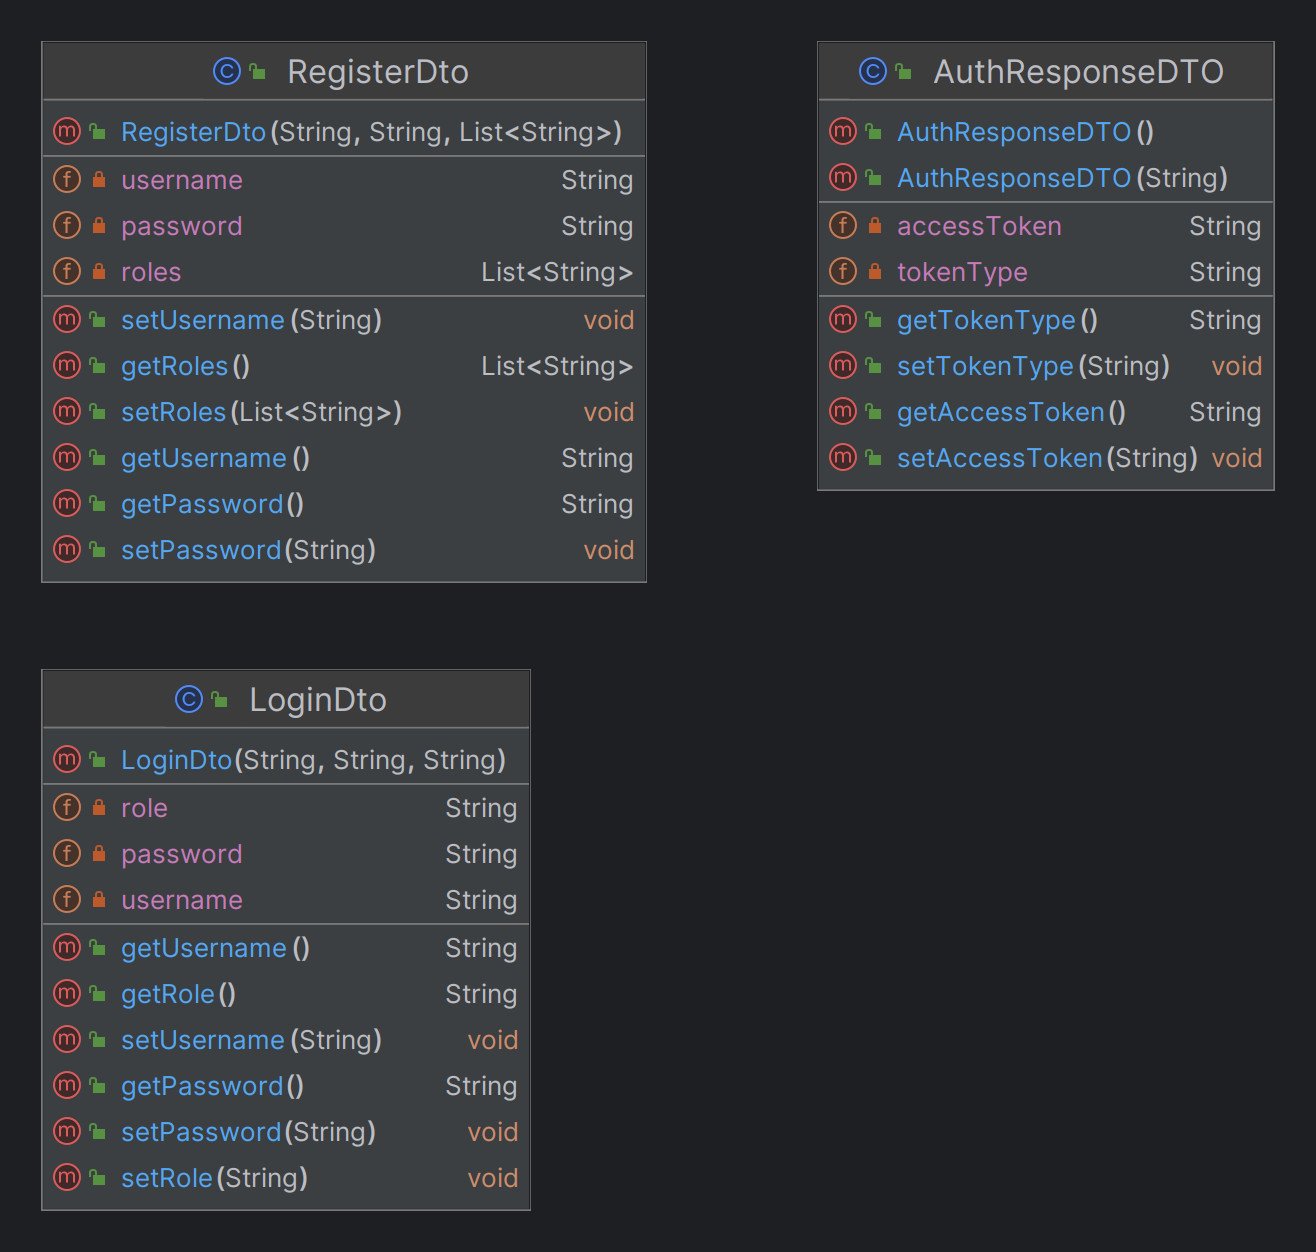
\includegraphics[width=0.9\textwidth]{slike/dtoUML}
				\caption{UML dijagram paketa \textit{DTO}}
				\label{fig:dtoUML}
			\end{figure}
			
			Slika 4.4 prikazuje paket \textit{Repository} koji preko JPA-a (\textit{Java Persistance API}) pristupa bazi podataka. Za stvaranje SQL upita koristi se \textit{Spring Data} koji omogućava kreirane metoda s posebnim imenima i iz njih stvara SQL upite. Primjerice \textit{findByUsername()} \textit{Spring Data} pretvara u SQL upit koji pretražuje tablicu \textit{Users} za određeno korisničko ime.
			
			\begin{figure}[htbp]
				\centering
				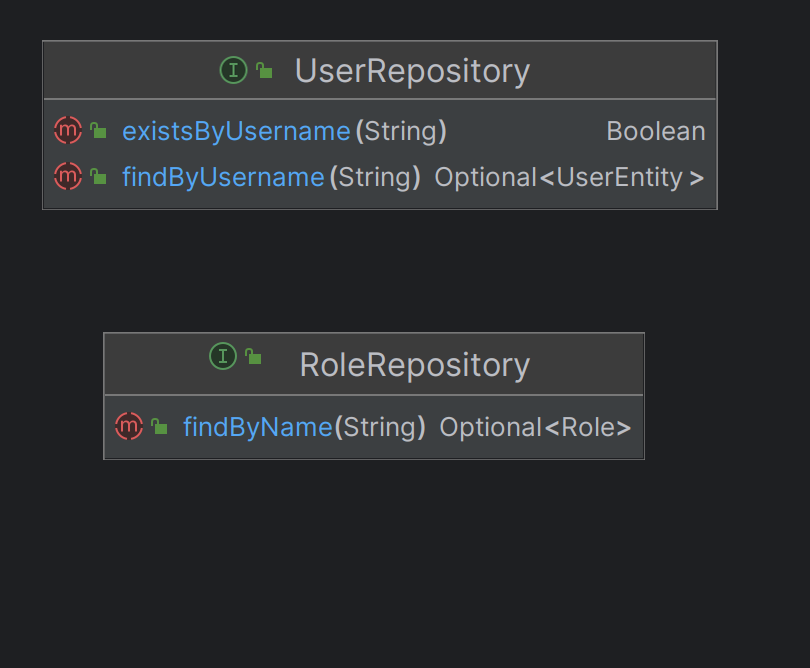
\includegraphics[width=0.9\textwidth]{slike/repoUML}
				\caption{UML dijagram paketa \textit{Repository}}
				\label{fig:repoUML}
			\end{figure}
			
			Slika 4.5 prikazuje paket \textit{Security} koji je zadužen za obradu svakog zahtjeva koji stiže na server i prosuditi ima li trenutni korisnik pravo pristupa. Glavna klasa za to je klasa \textit{SecurityConfig} koja preko metode \textit{filterChain()} primjenjuje filtre na svaki zahtjev da odredi pravo pristupa. Također klasa \textit{SecurityConfig} pomoću klasa \textit{JWTGenerator, JWTAuthenticationFilter i JwtAuthEntryPoint} za svaku uspješnu prijavu generira JWT token koji se zatim u svim zahtjevima tog korisnika koristi za autentifikaciju tog korisnika.
			
			\begin{figure}[htbp]
				\centering
				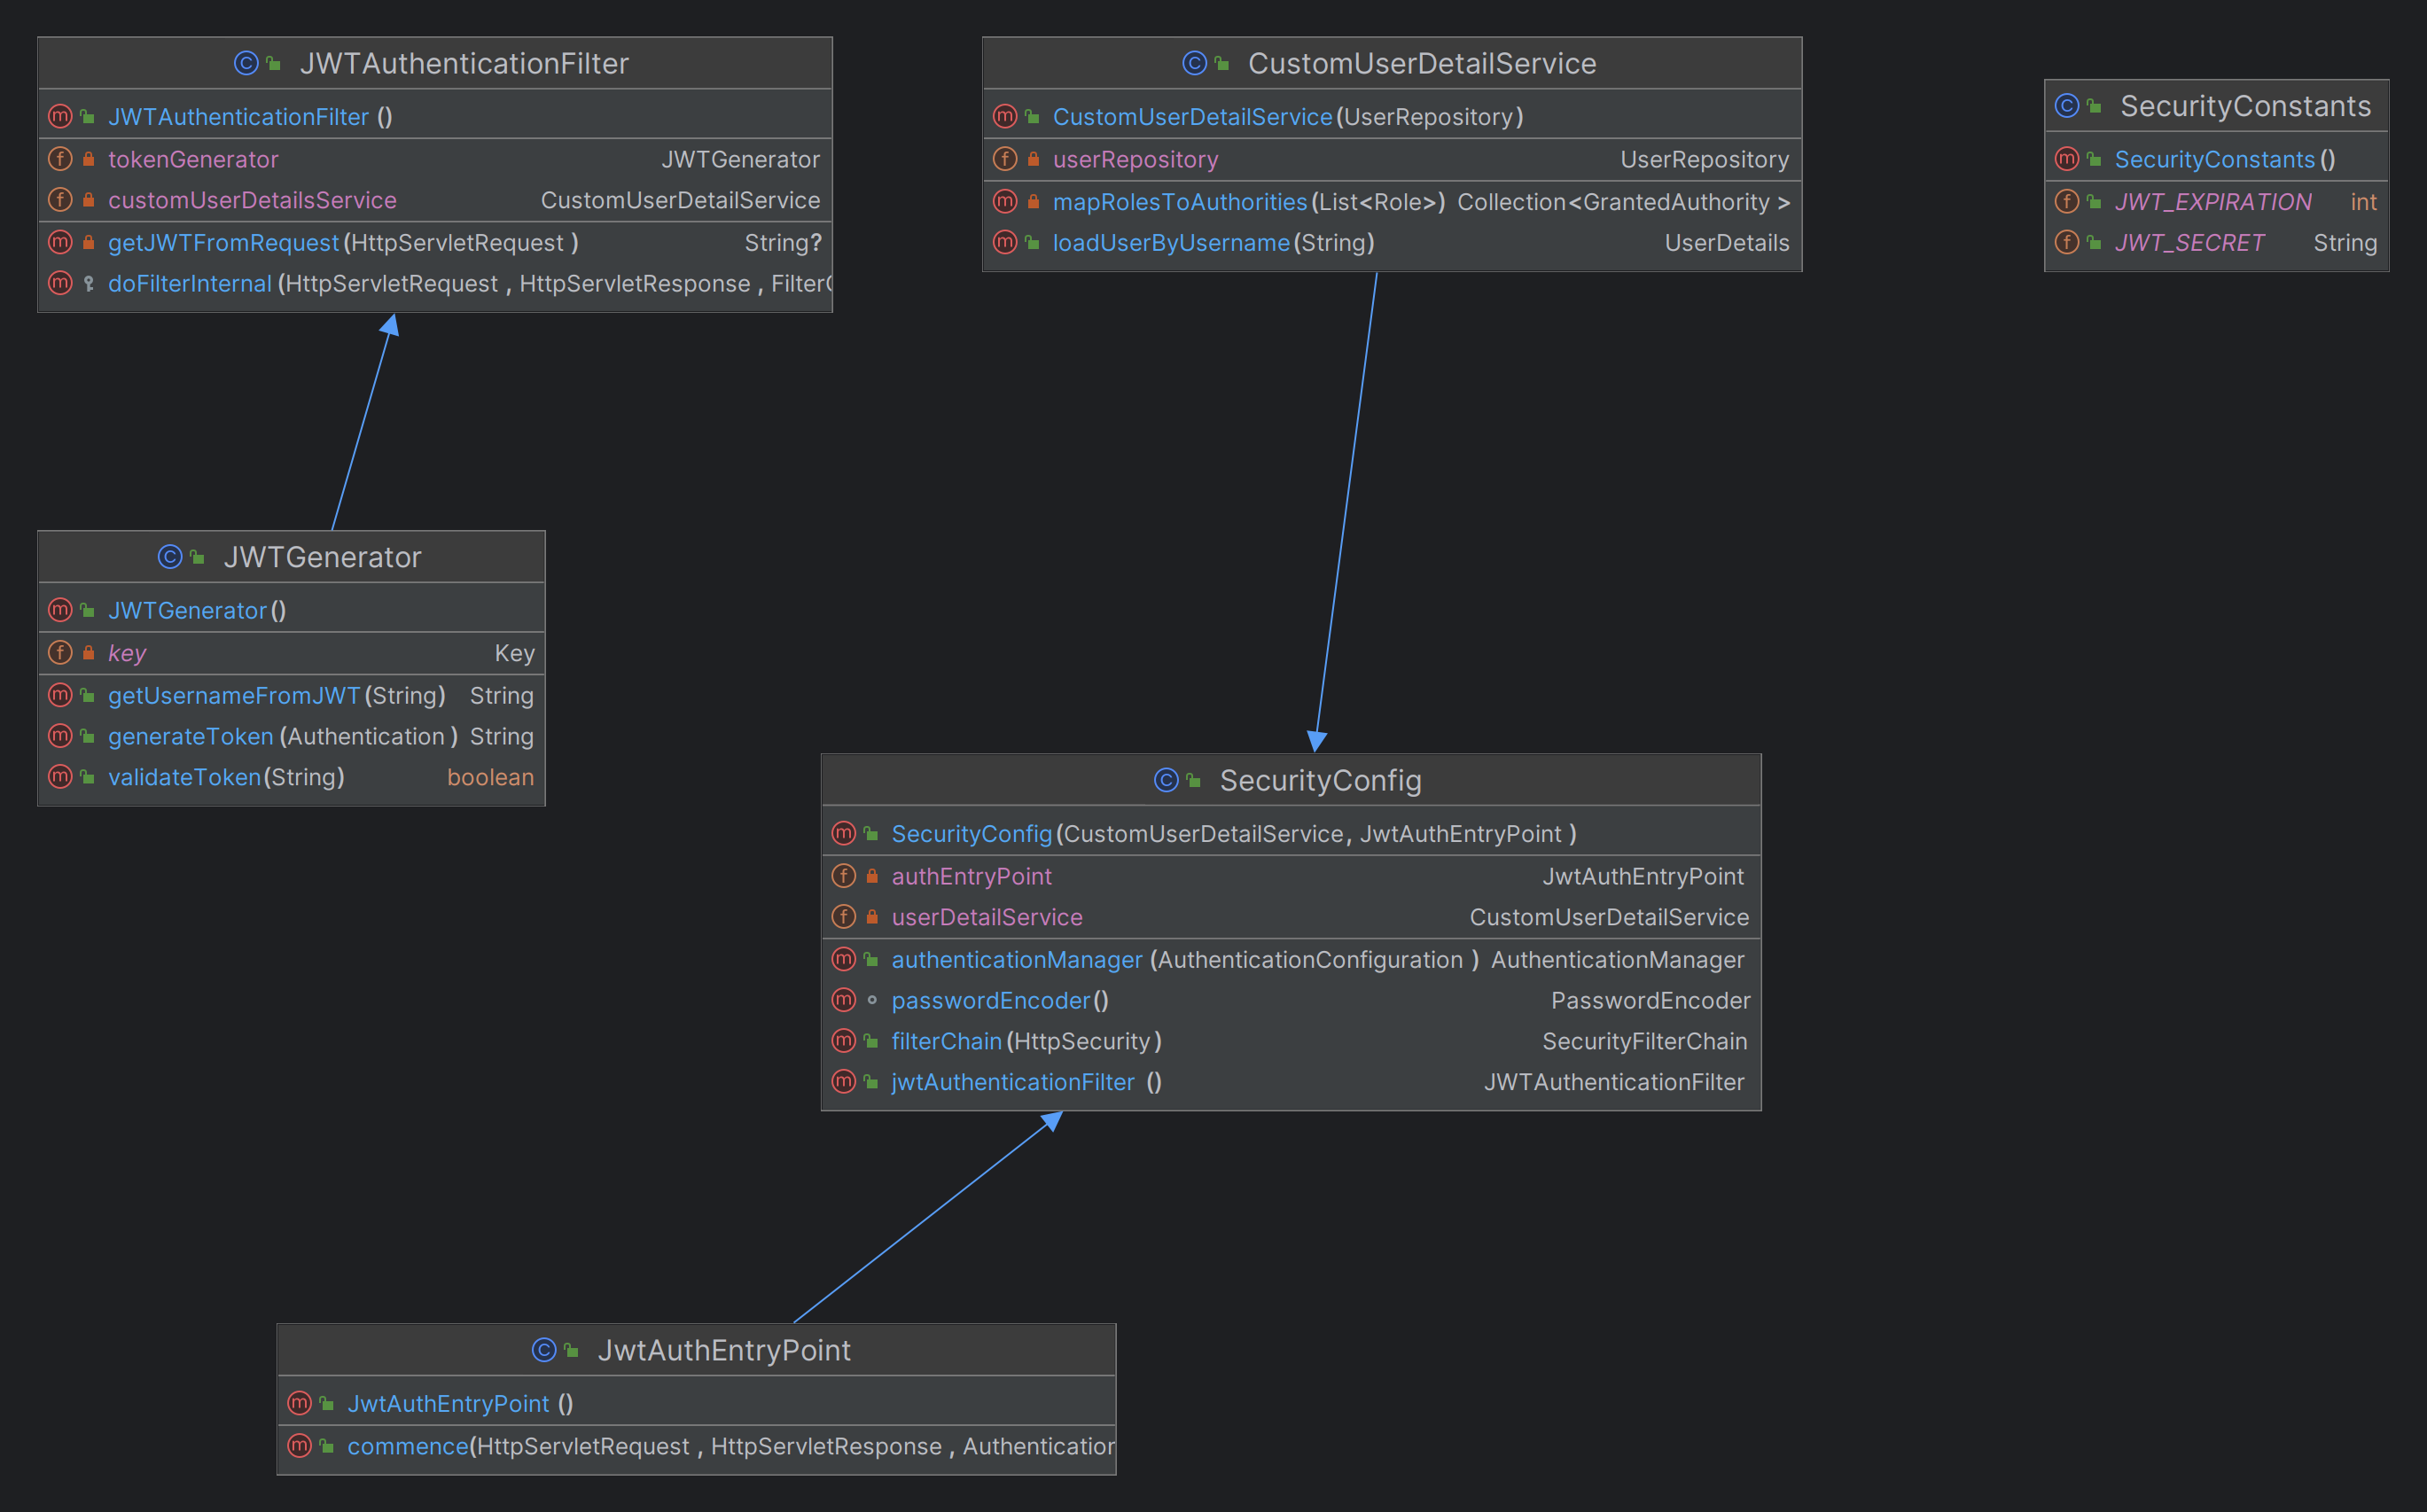
\includegraphics[width=0.9\textwidth]{slike/securityUML}
				\caption{UML dijagram paketa \textit{Security}}
				\label{fig:securityUML}
			\end{figure}
			
			
			
			\eject
		
		\section{Dijagram stanja}
			
			
			\textbf{\textit{dio 2. revizije}}\\
			
			\textit{Potrebno je priložiti dijagram stanja i opisati ga. Dovoljan je jedan dijagram stanja koji prikazuje \textbf{značajan dio funkcionalnosti} sustava. Na primjer, stanja korisničkog sučelja i tijek korištenja neke ključne funkcionalnosti jesu značajan dio sustava, a registracija i prijava nisu. }
			
			
			\eject 
		
		\section{Dijagram aktivnosti}
			
			\textbf{\textit{dio 2. revizije}}\\
			
			 \textit{Potrebno je priložiti dijagram aktivnosti s pripadajućim opisom. Dijagram aktivnosti treba prikazivati značajan dio sustava.}
			
			\eject
		\section{Dijagram komponenti}
		
			\textbf{\textit{dio 2. revizije}}\\
		
			 \textit{Potrebno je priložiti dijagram komponenti s pripadajućim opisom. Dijagram komponenti treba prikazivati strukturu cijele aplikacije.}